\documentclass{article}

\usepackage{fullpage}
\usepackage{graphicx}

\renewcommand*{\familydefault}{\sfdefault}

\begin{document}

% version 3b: 8MHz -> 12pF version, 2x 18p caps -> 2x 12p caps
% 47 discrete parts

% 16 resistors, 0603:
%   2x 22
%   4x 560
%   2x 1k
%   2x 4k7
%   2x 10k
%   3x 100k
%   1x 10M
% 19 capacitors, 0603:
%   4x 12p
%   9x 100n
%   3x 1u
%   2x 2u2
%   1x 4u7
% 2 crystals
% 2 switches
% 2 LEDs
% 6 other

\section*{Assembly guide and BOM for Micro Python PYBv3}

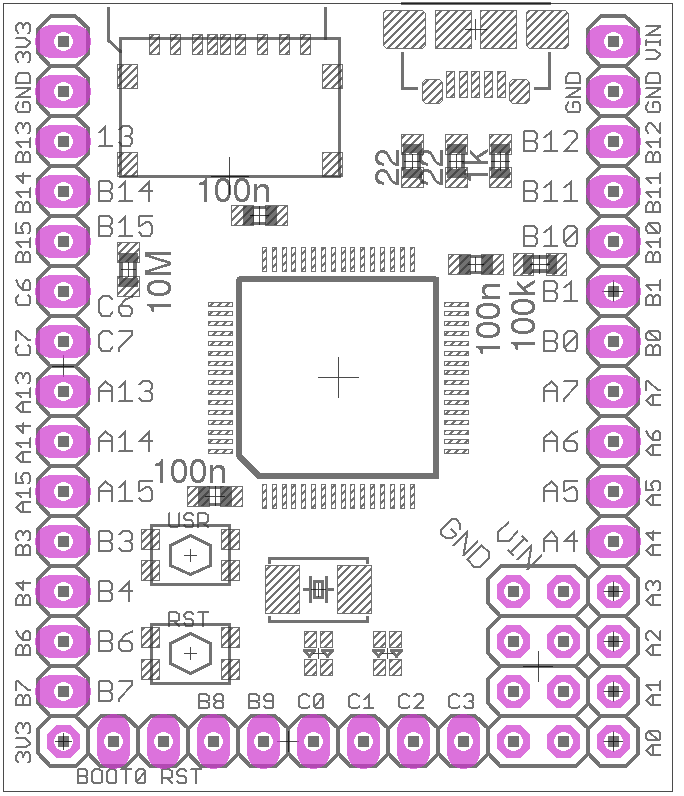
\includegraphics[width=0.49\textwidth]{topcomp}
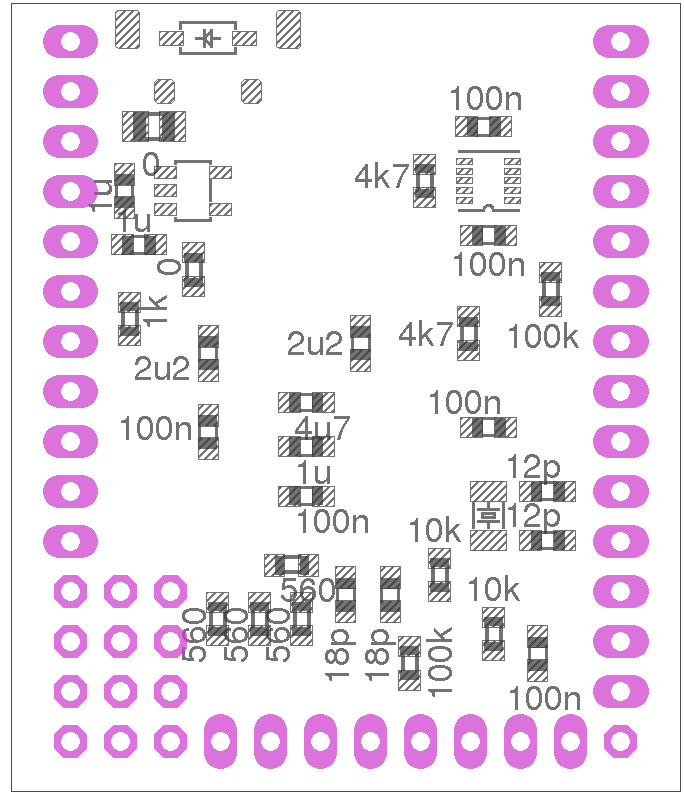
\includegraphics[width=0.49\textwidth]{botcomp}

\begin{center}
\begin{tabular}{|l|l|l|l|}
\hline

description & mfg part number & package & quantity \\
\hline\hline

microcontroller &
STM32F405RGT6 &
LQPF64 &
1
    
\\ \hline

3.3v LDO &
MCP1802T-3302I/OT &
SOT-23-5 &
1

\\ \hline

power diode &
1N5819HW-7-F &
SOD-123 &
1

\\ \hline

8MHz crystal &
7A-8.000MAAE-T &
SMT, 2 pads, 5x3.2mm &
1

\\ \hline

32kHz crystal &
9HT10-32.768KBZF-T &
SMT, 2 pads, 3.2x1.5mm &
1

\\ \hline

bicolour LED &
LTST-C195KGJRKT &
SMT, 4 pads, 1.5x1.6mm &
2

\\ \hline

accelerometer &
MMA7660F &
DFN-10 &
1

\\ \hline

micro SD socket &
1050270001 &
SMT, 9 pads, 11.24x7mm &
1

\\ \hline

USB micro-AB &
ZX62D-AB-5P8 &
SMT + through hole &
1  \\
&& 5 pads + 4 pins, 7.5x5.6mm  &

\\ \hline

push switch &
KMR421G LFS &
SMT, 4 pads, 5x2.8mm &
2

\\ \hline

resistor 22 & & 0603 & 2 \\
resistor 560 & & 0603 & 4 \\
resistor 1k & & 0603 & 2 \\
resistor 4k7 & & 0603 & 2 \\
resistor 10k & & 0603 & 2 \\
resistor 100k & & 0603 & 3 \\
resistor 10M & & 0603 & 1

\\ \hline

capacitor 12p & & 0603 & 4 \\
capacitor 100n & & 0603 & 9 \\
capacitor 1u & & 0603 & 3 \\
capacitor 2u2 & & 0603 & 2 \\
capacitor 4u7 & & 0603 & 1

\\ \hline\hline

total & & & 47 \\

\hline
\end{tabular}
\end{center}

\end{document}
